%
% Mathematical Representation of Networks
%

\section{Mathematical representation of networks}

\dropcap{W}{e} now turn our attention to defining a mathematical construction for the representation of (quantum and/or classical) networks, that we will subsequently rely on heavily in our framework for quantum networks. This encompasses representing networks as graphs, representing the cost of communications within the network, and how to optimise network routing to minimise costs.  These notions will be essential in our treatment of quantum networks.

%
% Graph-Theoretic Representation
%

\subsection{Graph-theoretic representation} \index{Network!Graphs}

We consider a classical network to be a weighted, directed graph,
\begin{align}\index{Network!Graphs}\index{Graphs}
	G=(V,E),
\end{align}
where vertices represent \textit{nodes} (\mbox{$v\in V$}) in the network, and the weighted edges represent communication \textit{links} (\mbox{$e\in E$}) between neighbouring nodes \cite{???}.

A node could be, for example, data storage, a classical computer implementing a computation, a router that switches the connections between incoming and outgoing links, or an end-user -- anything that communicates with the network, sender or receiver. A link on the other hand is any arbitrary means of communication between nodes, such as optical fibre, satellite, radio, electrical, smoke signals, tin cans connected by a taut piece of string, or well-trained carrier pigeon. In the protocols to be described here, it is completely irrelevant what the specific mediums for communication are. Rather what matters are \textit{costs} and \textit{attributes}, quantifying the relative performance of different links.

A key feature of the global internet is redundancy. In a packet-switched environment, sending identical packets twice might each follow entirely different routes to their common destination. Node-to-node redundancy is easily accommodated for in the graph-theoretic model by allowing multiple distinct edges between nodes. It is extremely important to accommodate multiple edges in network graphs, since redundant routes provide a direct means by which to load-balance a route. So, for example, a hub in Australia might connect to a sister hub in New Zealand using both a fibre-optic undersea cable, and simultaneously via a satellite uplink. If the faster of the two connections is running out of capacity, a proportion of the packets can simply be switched to the other link, thereby balancing the load. For this reason we abstain from using an adjacency matrix representation for network graphs, as they do not accommodate redundancy.

%
% Cost Vector Analysis
%

\subsection{Cost vector analysis} \label{sec:costs} \index{Cost vector analysis}\index{Attributes}

The edge weights in $G$ represent the \textit{costs} ($\vec c$) and \textit{attributes} ($\vec a$) associated with using that link. In general these needn't be single numbers, but would rather be sets or data-structures, representing different types of costs and attributes of links, of which there may be many. These could include, for example, latency, bandwidth, dollar cost, and quality measures.

The distinction between costs and attributes, is that costs may be expressed in terms of units which may be interpreted as distances metrics in a Euclidean sense, obeying the following requirements:

\begin{definition}[Network cost metrics] \label{def:metric} Cost metrics satisfy the properties:\index{Network!Cost metrics}
	\begin{itemize}
    	\item Identity operations: If a channel performs nothing, its associated cost is zero, \mbox{$c(\mathbb{\hat{I}}) = 0$}.
    	\item Triangle inequality: \\ $c(v_1\to v_2\to v_3) \leq c(v_1\to v_2) + c(v_2\to v_3)$, \\ across all paths \mbox{$v_1 \to v_2 \to v_3$}. In the case of strict equality under addition we refer to the cost as a \textit{strictly additive cost}.
    	\item Positivity: \mbox{$c\geq 0$}. This ensures that shortest-path algorithms will function correctly. It is also congruent with the intuitive expectation that data traversing a communications channel is not somehow better off than if it hadn't traversed that channel at all.
	\end{itemize}
\end{definition}
Attributes, on the other hand do not have a distance interpretation, and may have arbitrary structure. A detailed discussion on the relationship between costs and attributes is presented in Sec.~\ref{sec:c_vs_a}.

The reason we demand costs have a distance interpretation is so that graph-theoretic pathfinding algorithms (Sec.~\ref{sec:shortest_path}) are applicable, allowing us to build upon the vast pre-existing understanding of graph theory. Ideally we would like equality in costs' triangle inequality, which yields an exact cost. But often this isn't possible and we are satisfied with the inequality, which simply dictates an upper bound on cost.

A detailed discussion of some of the major costs and attributes that realistic quantum networks will be subject to is presented in Sec.~\ref{sec:quantum_meas_cost}.

A \textit{route}\index{Routes} between two nodes, Alice ($A$) and Bob ($B$), of the network, $G$, is an acyclic subgraph connecting those nodes, \mbox{$R_{A\to B}\subseteq G$}. In general ad hoc networks there will typically be multiple paths between two nodes \mbox{$A\to B$}. For a particular cost metric, the cost of an entire route is simply the sum of the costs of each of the constituent links,
\begin{definition}[Route costs]
The net cost of a route \mbox{$A\to B$}, using cost metric $c(A\to B)$, traversing nodes $v_i$, is,
\begin{align}\index{Route costs}
c(R_{A\to B}) = \sum_{i=1}^{|R_{A\to B}|-1} c(v_i \to v_{i+1}),
\end{align}
where $v_i$ is the $i$th node in the route $R_{A\to B}$.
\end{definition}

Fig.~\ref{fig:example_routes} illustrates a simple example network with all of its available routes, \mbox{$R_{A\to B} \subseteq G$}. Fig.~\ref{fig:simp_route_opt} illustrates the optimal path for \mbox{$A\to B$} based on edge weights.

\begin{figure}[!htbp]
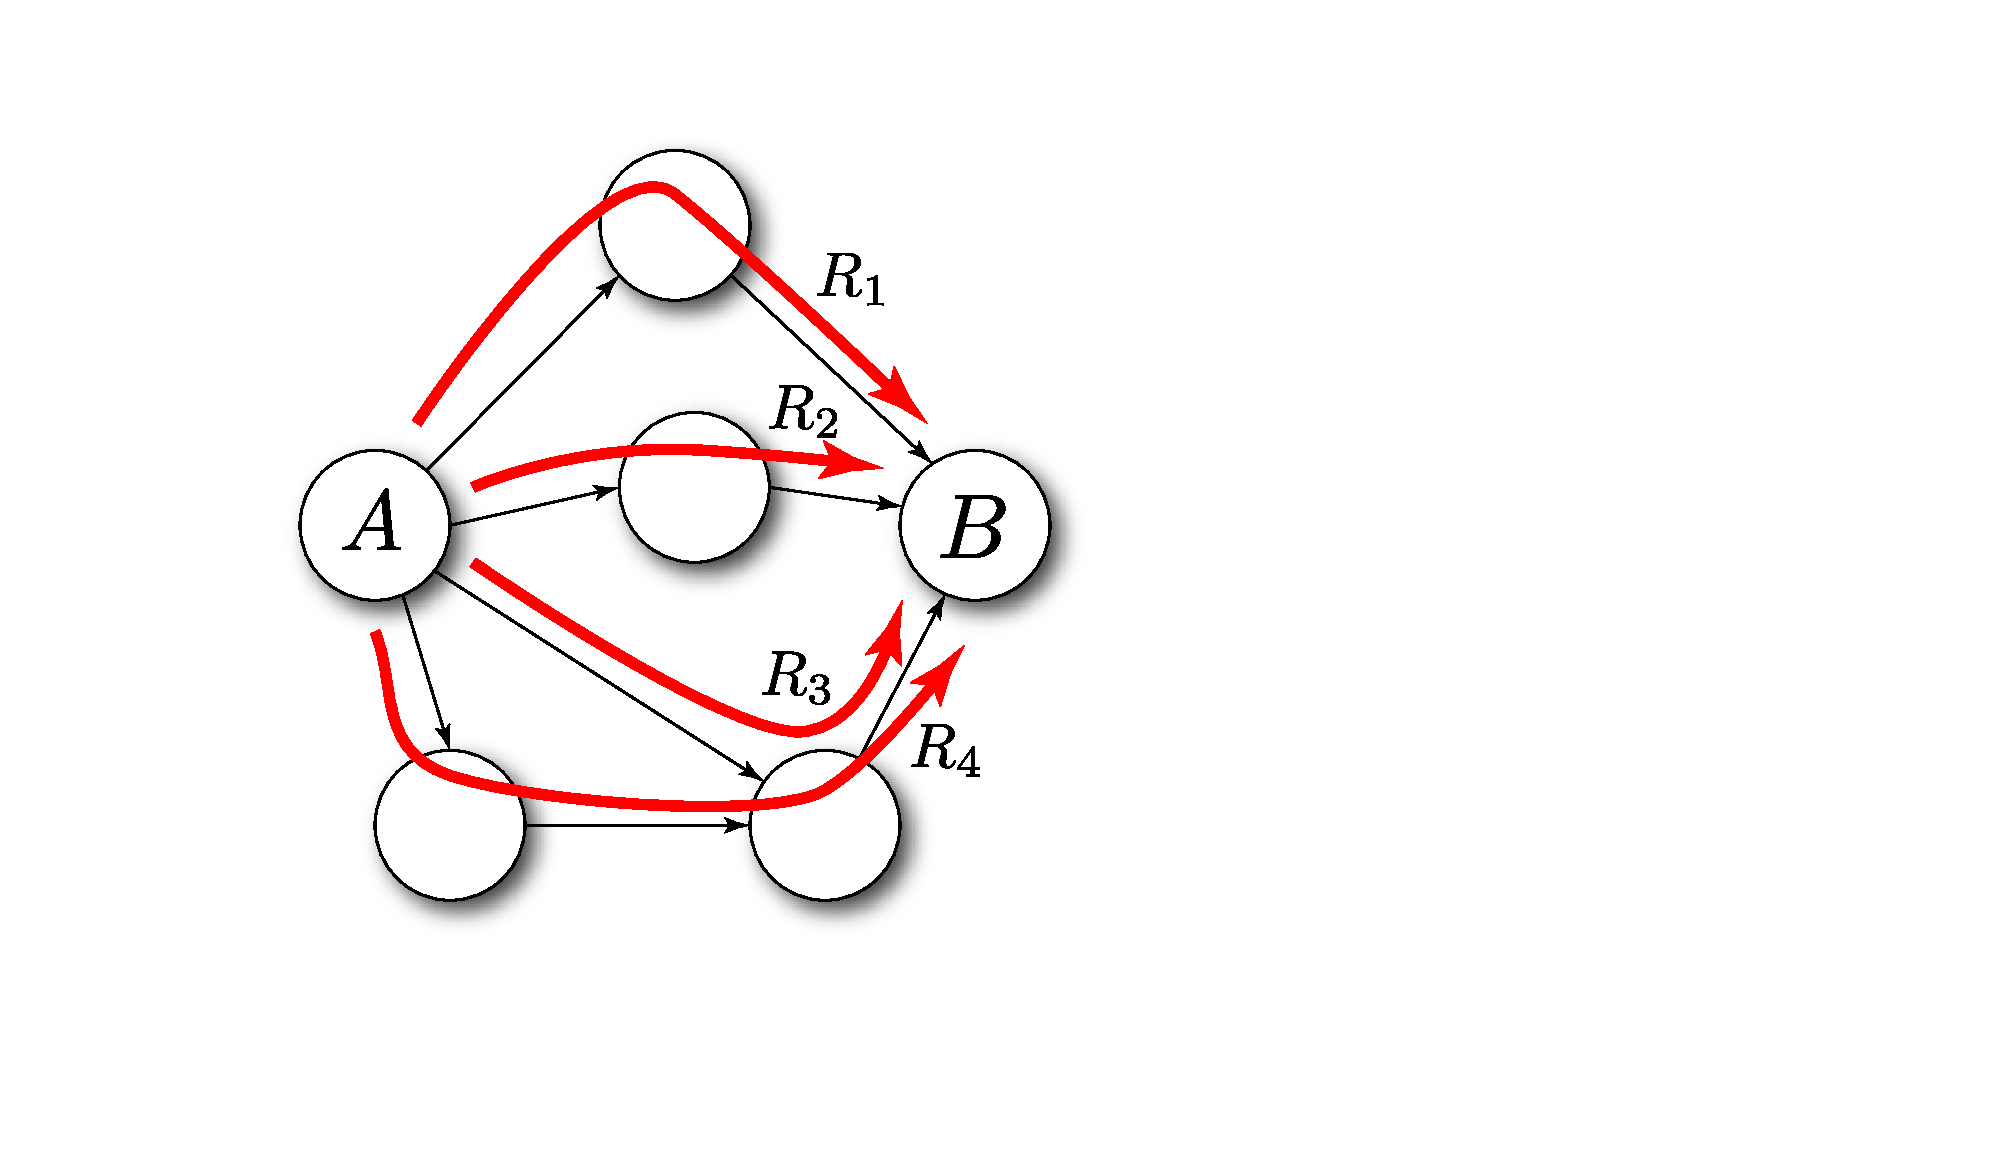
\includegraphics[clip=true, width=0.325\textwidth]{example_routes}
\captionspacefig \caption{Example of a simple network with multiple routes \mbox{$A\to B$}. Note that $R_3$ and $R_4$ are competing with one another for use of the last link, which the routing strategy, $\mathcal{S}$, will need to resolve if multiple simultaneous transmissions are taking place.} \label{fig:example_routes}
\end{figure}

\begin{figure}[!htbp]
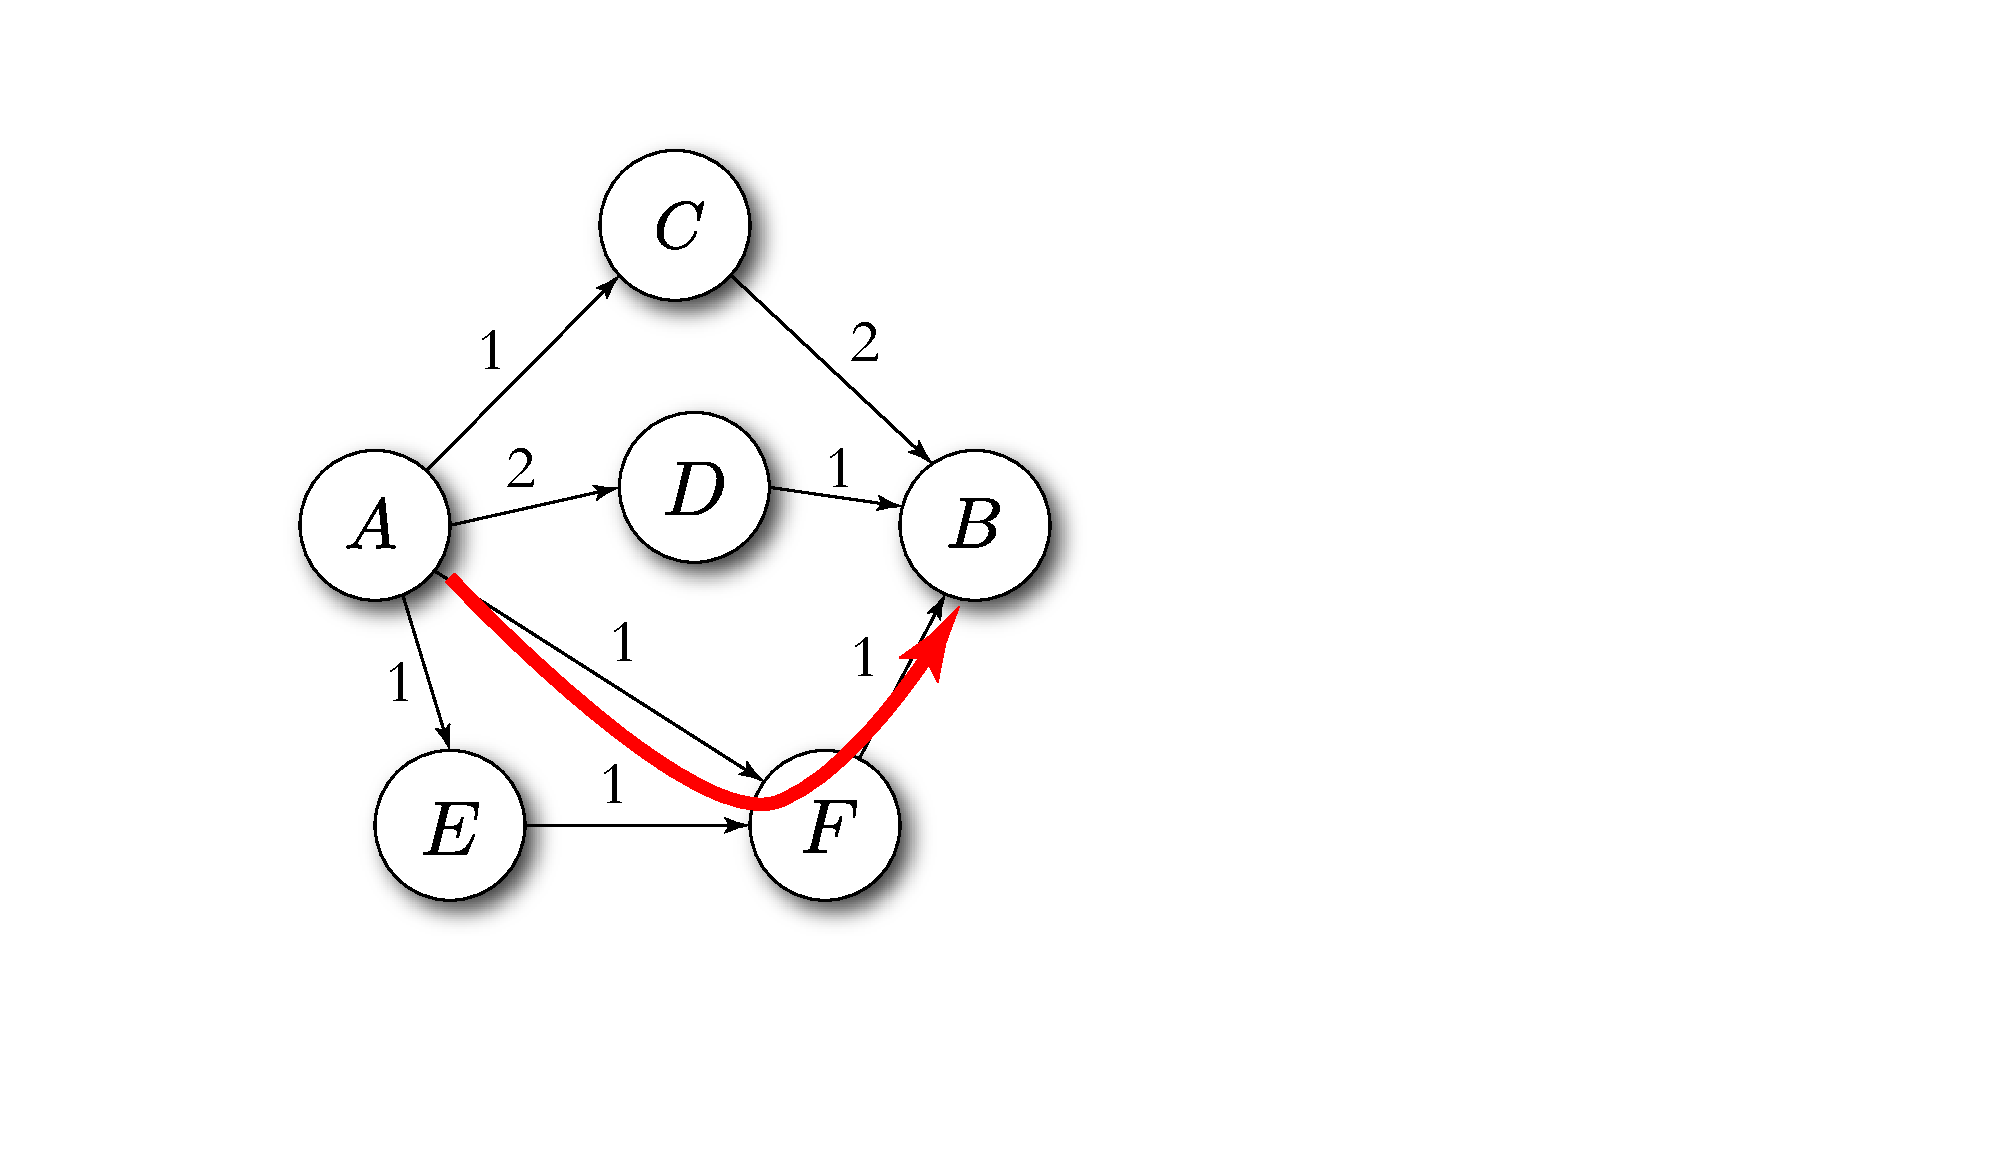
\includegraphics[clip=true, width=0.3\textwidth]{example_opt}
\captionspacefig \caption{The same network graph from Fig.~\ref{fig:example_routes}, with links weighted by some arbitrary cost metric. Applying a shortest-path algorithm yields the optimal route between Alice and Bob to be \mbox{$A\to F\to B$}, which incurs a net cost of \mbox{$c=2$}, as opposed to all other routes, which incur a net cost of \mbox{$c=3$}.} \label{fig:simp_route_opt}
\end{figure}

In a given network, it is unlikely that only a single cost metric or attribute will be of interest when determining optimal routings. There may be a tradeoff between different measures. For example, for time-critical applications the cost of a route might be considered a combination of both dollar cost and latency -- a satellite has very low latency but is extremely expensive, while a carrier pigeon is slow but cheap (and prohibited by PETA). What is the best tradeoff between the two?

To accommodate this, we allow the \textit{net cost} of a route to be defined as an arbitrary function of other primitive cost metrics and attributes of the route,
\begin{definition}[Net routing cost]\index{Net routing cost}
The net cost of a route \mbox{$A\to B$} is given by,
\begin{align} \label{eq:net_cost_R} \index{Net routing cost}
c_\mathrm{net}(R) = f_\mathrm{cost}(\vec{c}(R),\vec{a}(R)),
\end{align}
where $c_\mathrm{net}$ is a single numeric value representing the net cost as calculated from an arbitrary cost function, $f_\mathrm{cost}$, of the vector of associated costs and attributes.
\end{definition}
Note that the net routing cost needn't be a metric, as the cost function could be arbitrary. The net cost can be thought of as a ranking for routes, but not necessarily as a metric that accumulates across routes, since it already captures all these accumulations.

Eq.~(\ref{eq:net_cost_R}) gives us the net cost of a given route. For multiple users we would like to simultaneously optimise the cost across all users of the network. Thus we define the routing cost for the entire network to be,
\begin{definition}[Network routing cost]
	The net routing cost of all costs, over all active routes $\vec{R}$ is,
\begin{align} \label{eq:c_total}
c_\mathrm{total}(\vec{R}_{\vec{A}\to \vec{B}}) = \sum_{r \in {\vec R}_{\vec{A}\to \vec{B}}} c_\mathrm{net}(r),
\end{align}
where $\vec{R}_{\vec{A}\to \vec{B}}$ is a set of active routes connecting each pair \mbox{$A_i\to B_i~\forall ~ i$}.
\end{definition}

%
% Flow Networks
%

\subsection{Flow networks} \label{sec:flow_networks} \index{Flow networks}

On a shared network with many users utilising the network simultaneously, it may be the case that the preferred goal for the network is to maximise \textit{flow} \cite{???} -- the total amount of information that can be transmitted per unit time, i.e the net utilisation of the network's resources, summed over all users. In this case we can build on the existing theory of \textit{flow networks} \cite{???}, which characterise the load of links within the network.

A flow network is easily obtained from the network graph by associating a `capacity' attribute with each link and defining the graph weighted by the capacities as the flow network, preserving the underlying structure of the network graph.

When a route within the graph is utilised, we decrement the capacities of each link in that route, generating the so-called \textit{residual network} \cite{???}, which will now take the place of the original network in subsequent calculations. This process effectively tallies the links' utilisation, and when the tally hits zero, the link can no longer be used for any new routes. This forms a basic building block for more complex flow network algorithms.

There are many variations on flow networks. The simplest case is of a single user transmitting multiple packets simultaneously to a recipient. Depending on link capacities, different packets may need to follow different routes through the network, if network performance is to be maximised. Alternately, it may not be possible to send the desired number of packets simultaneously if the network capacity saturates.

The more complex (and realistic) scenario is of multiple users each transmitting from distinct starting nodes to distinct recipient nodes across a shared network. This is known as a \textit{multi-commodity flow network} \cite{???}, and is likely to be the dominant class of networks in real-world networking applications.

%
% Routing Strategies
%

\subsection{Routing strategies} \label{sec:route_strats} \index{Routing!Strategies}

A \textit{strategy}, $\mathcal{S}$, is simply an algorithm that chooses a route, based on the starting and finishing nodes of a communication, and also updates the vectors of costs and attributes within the network associated with the utilisation of that route,
\begin{definition}[Routing strategies]
A routing strategy is defined by,
	\begin{align}
\mathcal{S}(i,j,\vec{c},\vec{a}) &\to \{k,{\vec{c}}~',{\vec{a}}~'\}, \nonumber \\
i,j &\in V, \nonumber\\
k &\in \{R_{v_i\to v_j}\},
\end{align}
where $\mathcal{S}$ denotes the strategy, $k$ is a route, $i$ and $j$ are the source and destination nodes of the route, and $\vec{c}$ and $\vec{a}$ are vectors of associated costs and attributes.
\end{definition}
The goal of the strategy $\mathcal{S}$ is to minimise a chosen cost measure.

No particular route through a network is going to have infinite capacity, and therefore we cannot typically always reemploy the same most cost-effective route for all data. Particularly in multi-user networks, as routes are employed for communicating quantum states, their cost metrics may change according to load, or other external influences. Alternately, some routes may come into and out of operation. For example, a satellite requiring line-of-sight communication may oscillate in and out of sight, thereby periodically enabling and disabling respective network routes. For this reason, it is important that strategies accommodate dynamic changes in the network. This is easily accounted for by letting the edge weights in our network graph be a function of time, $G_t$, which are updated via the application of a strategy, which may also be time-dependent,
\begin{definition}[Time-dependent routing strategies]
A time-dependent strategy, $\mathcal{S}_t$, updates the network graph, $G_t$, at each time-step $t$,
\begin{align} \label{eq:S_G}
G_{t+1} = \mathcal{S}_t(G_t).
\end{align}
$S_t$ could be any \textbf{BPP} algorithm, deterministic or probabilistic.
\end{definition}
For example, the network might have bandwidth restrictions on some links, in which case if more than a certain amount of data is transmitted through a link, it is no longer available for use until previous transmissions have completed. Or, based on market dynamics, the dollar cost of utilising a link may change with its demand.

This type of cost minimisation approach to routing is analogous to \textit{distance-vector routing protocols}\index{Distance-vector routing protocols} in classical networking theory.

A detailed exposition of routing strategies is provided in Sec.~\ref{sec:strategies}.

%
% Strategy Optimisation
%

\subsection{Strategy optimisation} \label{sec:strat_opt} \index{Strategy!Optimisation} 

Clearly the goal when choosing routing strategies is to minimise the total cost, Eq.~(\ref{eq:net_cost_R}). That is, solving the optimisation problem,
\begin{definition}[Strategy optimisation]
The optimisation of strategies with a network comprising net costs $c_\mathrm{total}$ is given by,
\begin{align}
c_\mathrm{min} &= \underset{\mathcal{S}}{\mathrm{min}}(c_\mathrm{total}), \nonumber \\
\mathcal{S}_\mathrm{opt} &= \underset{\mathcal{S}}{\mathrm{argmin}} (c_\mathrm{total}).
\end{align}
\end{definition}

Choosing optimal strategies is a challenging problem, potentially requiring complex, computationally inefficient optimisation techniques. Strategy optimisation is an example of resource allocation, whose optimal solutions are often notoriously difficult to solve exactly, residing in complexity classes like \textbf{NP}-complete\index{NP \& NP-complete} (or worse!). In general, the number of possible routes through a graph will grow exponentially with the number of vertices. Thus, explicitly enumerating each possible route is generally prohibitive for large networks, unless some known structure provides `shortcuts' to optimisation. Having said this, Dijkstra's shortest path algorithm (discussed in Sec.~\ref{sec:shortest_path}) is the perfect counterexample, demonstrating that although an exponential number of routes may exist between two points, an optimal one can be found in \textbf{P}.

%
% Ad hoc Operation vs. Central Authorities
%

\subsubsection{Ad hoc operation vs. central authorities} \index{Central mediating authority} \index{Ad hoc networks}

When considering strategy optimisation, the first question to ask is `Who performs the optimisation, and who has access to what information?'.

In terms of who performs the optimisation, the two main options are that either each node is responsible for optimising the routes of packets passing through it (\textsc{Individual} algorithms), or there is a reliable and trusted central mediating authority\index{Central mediating authority} who oversees network operation and performs all strategy decision-making (\textsc{Central} algorithms).

In the case of \textsc{Individual} algorithms, the required knowledge of the state of the network could be obtained using network exploration algorithms (Sec.~\ref{sec:path_exp}) or gateway protocols (Sec.~\ref{sec:gateway}). 

On the other hand, for \textsc{Central} algorithms, either network exploration could be employed, or alternately the network policy could require nodes to notify the central authority upon joining or leaving the network. The former introduces an overhead in classical networking resource usage, since network exploration must be performed routinely to keep the ledger of nodes up-to-date. The latter, on the other hand, avoids this, but introduces a point of failure, in that all network participants must be reliable in notifying the central authority as required by the network policy. Failure to do so could result in invalid or suboptimal strategies.

%
% Local vs. Global Optimisation
%

\subsubsection{Local vs. global optimisation} \index{Local optimisation}\index{Global optimisation}

There are two general approaches one might consider when choosing strategies -- \textit{local optimisation} (\textsc{Local}) and \textit{global optimisation} (\textsc{Global}). \textsc{Local} simply takes each state to be communicated, one-by-one, and allows it to individually choose an optimal routing strategy based on the state of the network at that moment. \textsc{Global} is far more sophisticated and simultaneously optimises the sum of the routing costs, Eq.~(\ref{eq:c_total}), of all currently in-demand routes.

To implement \textsc{Local} optimisation, either \textsc{Individual} or \textsc{Central} algorithms may be employed. On the other hand, \textsc{Global} optimisation necessarily requires a \textsc{Central} algorithm, since it requires knowledge of the entire state of the network, which is collectively optimised.

Since \textsc{Global} represents the class of all algorithms that take all network costs by all packets into consideration, it must clearly perform at least as well as \textsc{Local}, which only takes into consideration the costs of a given packet. But we expect \textsc{Global} to perform better than \textsc{Local} in general, owing to the additional information it takes into consideration. We express this as \mbox{\textsc{Local}$\subset$\textsc{Global}}. However, \textsc{Global} requires solving a complex, simultaneous optimisation problem, which is likely to be computationally hard, whereas \textsc{Local} can be efficiently solved using multiple independent applications of, for example, an efficient shortest-path algorithm (so-called \textsc{Greedy} algorithms), discussed in Sec.~\ref{sec:shortest_path}.

A further stumbling block for \textsc{Global} is that it requires some central authority, responsible for the global decision-making, to have complete, real-time knowledge of the state of the entire network. This may be plausible for small LANs, but would clearly be completely implausible for the internet as a whole. So it is to be expected that different layers and subnets in the network hierarchy will employ entirely different strategy optimisation protocols. This is certainly reminiscent of the structure of the present-day internet.

Roughly speaking, we might intuitively guess that at lower levels in the network hierarchy, responsible for smaller subnets, there will be a tendency towards the adoption of \textsc{Global} strategies, as full knowledge of the state of the subnet is readily obtained and maintained. However, as we move to the highest levels of the network hierarchy (e.g routing of data across international or intercontinental boundaries), we might expect more laissez-faire (i.e \textsc{Greedy}) strategies to be adopted, since the prospects of enforcing a central authority with full knowledge of the state of the internet, who is also trusted by all nations to fairly and impartially allocate network resources and mediate traffic, is highly questionable.

We will not aim to comprehensively characterise the computational complexity of \textsc{Global} strategies. However, in Sec.~\ref{sec:strategies} we will present some elementary analyses of several toy models for realistic strategies. Some such strategies are efficient although not optimal, but nonetheless satisfy certain criteria we might expect.

Future developments in the optimisation techniques required for \textsc{Global} strategies may improve network performance, leaving our techniques qualitatively unchanged.

When employing \textsc{Local}, on the other hand, things are often far simpler. If we are optimising over a cost metric satisfying the distance interpretation, we may simply employ a shortest-path algorithm to find optimal routes through the network.

If one were to become even more sophisticated, one might even envisage treating network resource allocation in a game theoretic context \cite{???}, which we won't even begin to delve into here.

%
% Message- vs. Packet-Level Routing
%

\subsection{Message- vs. packet-level routing}

In Eq.~(\ref{eq:S_G}) we defined the action of a strategy, $\mathcal{S}$, on a network, $G$. However, we were intentionally ambiguous in our introduction of the time-dependence, given by $t$. This is to allow us to consider changes at one of two different time-scales: the packet level, or the message level. The \textit{message} is the entire data stream transmitted from Alice to Bob, whereas the \textit{packet} is a small block of data taken from the message, where each packet may be independently routed.

When defining the action of strategies, we could do so at either of these time-scales. We could choose routes in their entirety, from start to finish, at the beginning of the message transmission, under the assumption that the costs in the network will be constant over that duration and no one will misbehave. We refer to such strategies as \textit{message-level strategies}. Alternately, and perhaps more realistically in many scenarios, the costs and attributes of a network could be highly dynamic and readily change within the transmission time-window. In that case, we will employ \textit{packet-level strategies}, which reevaluate the strategy independently for each packet and for each of their hops between nodes.

In our future discussions on routing strategies, context will make it clear when we are referring to packet- or message-level strategies.